\documentclass[12pt,a4paper]{article}

\usepackage[utf8]{inputenc}
\usepackage[T1]{fontenc}
\usepackage[french]{babel}

\usepackage{amsmath, amssymb}

\usepackage{graphicx}
\usepackage{caption}

\usepackage{siunitx} % Pour les unités

\usepackage{geometry}
\geometry{top=2cm, bottom=2.5cm, left=3cm, right=3cm}
\setlength{\parindent}{0pt}

\usepackage[sfdefault]{roboto}

\usepackage{enumitem}

\usepackage{hyperref}

\usepackage{xcolor}

\usepackage{multicol}
\setlength{\columnseprule}{1pt}
\def\columnseprulecolor{\color{gray}}

\usepackage{tcolorbox}


\usepackage{import}
\usepackage{xifthen}
\usepackage{pdfpages}
\usepackage{transparent}
\usepackage{float}

\newcommand{\incfig}[1]{%
	\def\svgwidth{\columnwidth}
	\import{./figures/}{#1.pdf_tex}
}


\newcommand{\RomanNum}[1] %pour les chiffre romain
{\MakeUppercase{\romannumeral #1}}











\title{Modélisation}
\author{}
\date{\today}

\begin{document}
	\counterwithin{section}{part} % pour que \section{} recommence de 1 aprés \part{}
	
	
	\tableofcontents
	
	\newpage
	
	\part{TP N01}
	
	\section{Définitions}
	
	\begin{itemize}
		\item $A_{0}$ : Aire de la section homogénisé.
		\item $M_{s}$ : Moment fléchissant max a l'ELS.
		\item $E_{v}$ : Module de déforamtion différée du béton.
		\item $E_{i}$ : Module de déforamtion instantanée du béton.
		\item $I_{fi}$ : Moment d'inertie fictif pour les déformations de longue durée.
		\item Moment d'inertie fictif pour les déformations de instantanée.
		\item $\rho$ : Le rapport de l'aire A dans les sections des armatures tendues a l'aire de la section utile de la nervure.
	\end{itemize}
	
	\section{Calcul de la fléche}
	
	\[ \begin{cases}
		f_{i} = \dfrac{M_{s} \cdot l^{2}}{10 \cdot E_{i} \cdot I_{fi}} \quad\leq\quad \overline{f_{i}}=\dfrac{l}{500} \\\\
		f_{v} = \dfrac{M_{s} \cdot l^{2}}{10 \cdot E_{v} \cdot I_{fv}} \quad\leq\quad \overline{f_{v}}=\dfrac{l}{500}
	\end{cases} \]
	
	
	
	\subsection{Aire de la section homogénisie (Acier + béton)}
	
	\[ A_{0} = A+n \cdot A_{st} \quad \text{Avec : } n = 15 = \dfrac{E_{acier}}{E_{béton}} \]
	
	
	
	\subsection{Le moment statique de la section homogénisie}
	
	Moment statique par rapport a \underline{\textbf{x-x'}} 
		
	\[ S/_{xx'} = \dfrac{b \cdot h^{2}}{2}+ 15 \cdot A_{st} \cdot d \]
	
	Supposont en travée que $A_{st} = 3HA10 = 2,35~\unit{cm^{2}}$.
	
	
	\subsection{Position du centre de gravité}
	
	\begin{figure}[H]
		\centering
		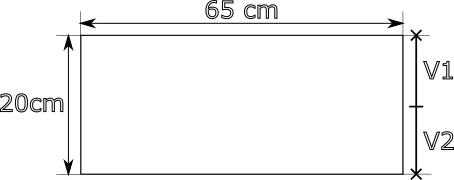
\includegraphics[width=0.5\linewidth]{figures/section-T-rectangulaire}
		\caption{}
		\label{fig:section-t-rectangulaire}
	\end{figure}
	
	
	\[ V_{1} = \dfrac{S/_{xx'}}{A_{0}} \]
	
	\[ V_{2} = h - V_{1} \]
	
	
	
	\subsection{Moment d'inertie de la section homogénisé}
	
	Moment d'inertie par rapport au CDG
	
	\begin{figure}[H]
		\centering
		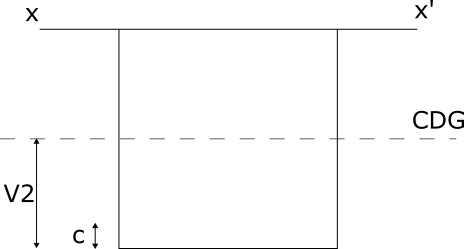
\includegraphics[width=0.5\linewidth]{figures/section-T-rectangulaire2}
		\caption{}
		\label{fig:section-t-rectangulaire2}
	\end{figure}
	
	\[ I_{0} = \dfrac{b}{3} \cdot (V_{1}^{3}+V_{2}^{3})+ 15 \cdot A_{st} \cdot (V_{2}-c)^{2} \]
	
	
	\subsection{Calcul des interies fictives}
	
	
	
	\[ I_{fi} = \dfrac{1,1 \cdot I_{0}}{1 + \lambda_{i} \cdot \mu} \hspace{2cm}
	I_{fv} = \dfrac{1,1 \cdot I_{0}}{1 + \lambda_{v} \cdot \mu}
	\]
	
	
	
	\[ \rho = \dfrac{A_{st}}{b \cdot d} \]
	
	\begin{figure}[H]
		\centering
		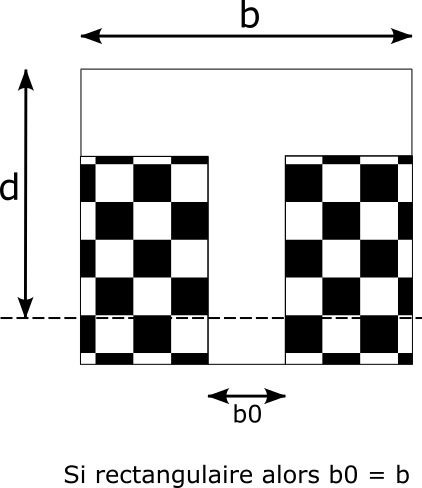
\includegraphics[width=0.3\linewidth]{figures/section-T-rectangulaire3}
		\caption{}
		\label{fig:section-t-rectangulaire3}
	\end{figure}
	
	
	\[ \lambda_{i} = \dfrac{0,05 \cdot f_{t28}}{\rho \cdot \left( 2+\dfrac{3 \cdot b_{0}}{b} \right)} \]
	
	\[ \lambda_{v} = \dfrac{2}{5} \cdot \lambda_{i} \]
	
	\vspace{\baselineskip}
	
	\[ \mu = 1 - \dfrac{1,75 \cdot f_{t28}}{4 \cdot \rho \cdot \overline{\sigma}_{st} \cdot f_{c28}} \]
	
	
	
	
	\subsection{Calcul des fléches}
	
	\subsubsection{Module d'élasticité(déformation) du béton}
	
	\[ E_{i} = 11000 \cdot \sqrt[3]{f_{cj}} \hspace{2cm} E_{v} = 3700 \cdot \sqrt[3]{f_{cj}} \]
	
	\subsubsection{Fléches}
	
	\[ \begin{cases}
		f_{i} = \dfrac{M_{s} \cdot l^{2}}{10 \cdot E_{i} \cdot I_{fi}} \quad\leq\quad \overline{f_{i}}=\dfrac{l}{500} \\\\
		f_{v} = \dfrac{M_{s} \cdot l^{2}}{10 \cdot E_{v} \cdot I_{fv}} \quad\leq\quad \overline{f_{v}}=\dfrac{l}{500}
	\end{cases} \]
	
	
	
	
	
	
	
	
\end{document}